\documentclass[11pt]{article}
\usepackage{amsmath}
\usepackage{graphicx}
\usepackage[margin = 1.22 in]{geometry}
\graphicspath{ {images/} }
%opening
\title{Properties of Damped Oscillations}
\author{Andy Badea, Alexander Hoerler, Eashwar Mahadevan, Victor Zhao}

\begin{document}

\maketitle
\begin{center}
	\begin{tabular}{l r}
		Date Performed: & November 27, 2017 \\ % Date the experiment was performed
		Instructor: & Dr. Bradley Miller % Instructor/supervisor
	\end{tabular}
\end{center}
\section{Introduction}
Suppose one has a mass resting on the end of a spring, the other end of which is fixed in place. Several things might happen. The spring might be in its equilibrium position, in which case the mass would not move. Alternatively, the spring might be over-compressed, in which case the spring, seeking to relieve its tension, would extend and accelerate the mass towards equilibrium. The spring may also be overextended, in which case the spring would retract, once again accelerating towards equilibrium. However, even with this perpetual acceleration toward equilibrium, the mass and spring still find it difficult to come to rest. Instead, the mass, seeking to reach equilibrium, overshoots and must be once again drawn back. If allowed to move freely, the spring will bob back and forth. The spring will oscillate. Oscillations are a type of motion which is periodic, meaning it repeats in a predictable pattern. Objects like pendulums and springs can experience oscillations. In the simplest of cases, the oscillator will return exactly to its initial condition after one period. However, this is not always the case. The motion of these oscillators may be affected when the spring’s motion is damped — being resisted in some way proportional to the speed at which the mass moves. The source of the damping usually comes from some kind of spring friction. This damping causes the oscillator to slow down, and thus means that the amplitude reach in progressive periods will be smaller. The elasticity constant of a spring, mass on the end of a spring, and the damping constant all affect the motion of the spring’s oscillation. The damping constant will affect the rate at which the oscillator’s amplitude decreases. If the damping constant is very large, the oscillator will begin to swing at rather small amplitudes rather quickly, while if the opposite is the case the amount after a long time will be rather similar to the initial amplitude. Therefore, working backwards, the damping constant may be found by analyzing the motion of oscillators over a period of time. In this lab, that relationship will be found and the angular velocity will also be found using the movements of the spring.
\section{Procedure}	
In this experiment a spring/clamp apparatus was constructed from which the oscillator would hang. A clamp was attached to the side of a lab workstation. A paper clip was then attached the side of the clamp. A spring was hung from the paper clip, with a hanging mass hung from the other end of the spring. A ring stand apparatus was constructed by attaching an o-ring to the stand and placing a wire mesh on top of the ring clamp in order to protect the motion sensor from falling objects. The motion sensor was placed on the base of the stand so that it was directly under the hanging mass and protective mesh. First, the spring constant of two springs was calculated by placing slotted masses ranging from 100.0 g to 900.0 g on the spring and measuring the displacement. Approximately 4-5 trials were taken for each spring. After calculating the spring constant, the spring was attached to the clamp apparatus, and a mass was hung on the end of the spring. The spring and hanging mass were held such that the spring was in its natural equilibrium position, then the hanging mass was  dropped in such a way so that there was little sway in the bouncing spring and data collection was started. The distance of the mass to the motion sensor was measured continuously for 30 seconds of damped oscillation for each trial. Four separate spring/mass combinations were used. This was repeated with the same 4 spring/mass combinations and an index card (m = 2.02g) taped to the bottom of the hanging mass, altering the damping constant of the oscillation.
\begin{figure}[h]
	\caption{The mass would bob above and below its equilibrium position.}
	\centering
	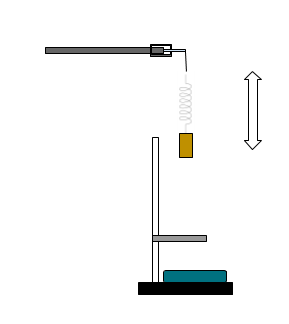
\includegraphics[width=2in, height=2 in]{Diagram}
\end{figure}

\section{Data}
The first data collection involved finding the physical properties of the system. The spring constant of both of the two springs was found by placing different masses on the bottom of the spring and measuring their extension. 
\begin{figure}[h]
	\centering
	\begin{tabular}{|c|c|c|c|c|c|}
		\hline 
		\multicolumn{3}{|c|}{Spring 1} & \multicolumn{3}{|c|}{Spring 2}\\
		\hline 
		Mass & Force & Displacement & Mass & Force  & Displacement  \\
		(g) & (N) & (cm) & (g) & (N) & (cm) \\
		\hline 
		20.0 & 0.196 & 1.06 & 400.0 & 3.92 & 0.80 \\ 
		\hline 
		50.0 & 0.490 & 2.63 & 500.0 & 4.90 & 1.76 \\ 
		\hline 
		100.0 & 0.980 & 5.44 & 600.0 & 5.88 & 2.76 \\ 
		\hline 
		150.0 & 1.47 & 8.11 & 700.0 & 6.86 & 3.82 \\ 
		\hline 
		200.0 & 1.96 & 10.79 & 1000.0 & 9.80 & 6.92 \\ 
		\hline 
	\end{tabular} 
\end{figure}
\\
If these points are graphed, the slopes of the lines represent the spring constants of the two springs. The first was found to be \(18.07 \pm 0.10 \; \mathrm{N}/\mathrm{m} \) while the second was found to be \(95.7 \pm 0.8 \; \mathrm{N}/\mathrm{m} \). One may see these graphs on the attached graph page.

The motion of each of the oscillators was recorded with the motion sensor. The graphs of this as well as the curve fit and its parameters are on the attached graph pages. One should note that the fits of the curves are very tight, with \(r^2\) values well into 99\%s. This means that the model for damped harmonic motion reached in the analysis (See next section) accurately models the physical phenomenon.  
\section{Analysis}
Let’s suppose we have a mass on the end of a spring resting off the end of the table. The mass will Suppose there is a mass at the end of a spring which resting off the edge of the table. The mass has relatively few forces acting upon it. One of these forces is the result of gravity, which draws the mass down towards the earth. This force will simply be \(- m \, g\) where \( m \) is the mass of the mass allowed to rest at the base of the spring and \( g \) is the acceleration due to gravity. The spring will naturally exert a force on the spring. This force is proportional to the negative distance of the mass to the spring’s equilibrium position. We may express this force as \( - k \, x \), where \( k \) is the spring constant and \( x \) is the distance that the spring has been extended. There is one remaining force that will model the damping that the mass experiences. We will imagine some force slowing the mass down that is proportional to the speed at which the mass moves. We will express this as \( - b \, x^{\prime}(t)\) where \(b\) is some constant related to the damping and \(x^{\prime}(t)\) the speed of the mass. Thus the forces on the mass at any given time may be written as
\[ F = - m \, g - k \, x - b \, x^{\prime}(t) \]
Of course we recall that by Newton's second law of motion, \(F = m \, a\), the force may be substituted by the product of the mass and the acceleration.
\[ m \, a = - m \, g - k \, x - b \, x^{\prime}(t) \]
We may write this such that the terms all fall on one side, and for consistency with the remainder of the equation replace the term \(a \) with \(x^{\prime\prime}(t)\). This leaves us with the simple differential equation.
\[ m \, x^{\prime \prime}(t) + b \, x^{\prime}(t) + k \, x  + m \, g  = 0\]
One might solve this by converting the above differential equation into its characteristic equation.
\[m \, r^2 + b \, r + k = 0 \]
This is rather simple to solve, and may be done as a simple quadratic equation.
\[ r  = \frac{-b}{2 \,m} \pm \frac{\sqrt{4 \, m k - b^2}}{2 \, m} i\]
Of course the solutions are almost certainly not real but, this is what gives simple harmonic oscillations their characteristic sinusoidal motion.\footnote{Note that the solutions are only imaginary if \( b^2 - 4mk < 0\). This only occurs in underdamped oscillation which is what was measured.} Now, with this information it is relatively easy to model the position \(x(t)\) without much effort. The any sum of these two 
\[ x(t) = c_1 \, \mathrm{e}^{r_1} + c_2 \, \mathrm{e}^{r_2} - \frac{m \, g}{k}\]
Where \(r_1\) and \(r_2\) are the two solutions to the characteristic equation.  is often useful to us to separate \(r\) into its real and imaginary parts. The real part of \(r\) is the rather simple to find, \(b/2m\). The imaginary part remain a little bit more complicated, we will refer to the imaginary portion of the solutions as \(\pm \omega\) for reasons that will hopefully become clear. This allows us to rewrite the expression.
\[ x(t) = c_1 \, \mathrm{e}^{-bt/2m} \, \mathrm{e}^{ i \omega t} c_2 \, \mathrm{e}^{-bt/2m} \, \mathrm{e}^{ i \omega t} - \frac{m \, g}{k}\]
Both sides of the sum, that with \(c_1\) and with \(c_2\)  have a \(e^{-bt/2m}\) term which may be factored out. The remaining portions, those with imaginary exponents are sine waves and thus so is there sum. They will have a sum with some amplitude \(A\) and some phase \(\phi\). This rids us of the need to use the constants \(c_1\) and \(c_2\)
\[ x(t) =A \, \mathrm{e}^{-bt/2m}\, \sin(\omega \, t + \phi) - \frac{m \, g}{k} \label{eq:1} \]
If one measures the position of one of these damped as a function of time, one may try to fit such a curve onto the data. The most function to fit is of the form.
\[x(t) = A \mathrm{e}^{-B t} \, \sin(C \, t + D) + E\]
Each of these parameters have a meaningful physical interpretation. \(A\) represents the initial amplitude of the oscillation. If the mass was dropped from rest (it was) this value represents the distance from its initial potion to its equilibrium position. \(B\)’s value is a little bit more involved. As in equation \eqref{eq:1}, the exponent is \(b/2m\). \(B\) is proportional to the damping force and inversely proportional to the mass of the object. \(C\) is the same as \(\omega\), the angular speed. This may be calculated as a function of \(b\), \(m\), and \(k\) . \(D\) represents the phase shift. This should represent the position at which the mass begins. In reality the masses were all released from the top of their period, but the beginning of the data collection period did not necessarily coincide with the beginning of the oscillation and thus \(D\) has rather little meaning in this context. The final parameter \(E\) represents the average position of the mass. This ought to be the height of the bottom of the mass on the unextended spring to the distance sensor minus the elongation of the spring when it is in equilibrium, \(m \, g / k\).

We may calculate the damping coefficient for the two situations (with and without index card) by comparing the calculated parameter \(B\) with mass, \(m\), recall that
\[ B = \frac{b}{2m} \].
Solving for b,
\[ b = \frac{B}{2m}\]

Likewise we may try to  find angular speed function of both the parameters and the measured physical properties of the system.

\[C = \omega = \frac{\sqrt{4 \, m \, k - b^2}}{2 \, m}\]

\subsection{Error Propagation}
In order to represent the error in the measurement of the damping constant. One might find the  error contribution with respect to each parameter simply by taking partial derivatives with respect to each parameter.
\[\frac{\partial b}{\partial B} = \frac{b}{B} \]
\[\frac{\partial b}{\partial m} = - \frac{b}{m} \]
This means that the total error in \(b\) may be expressed as
\[ \delta_b = b \sqrt{\left(\frac{\delta_B}{B}\right)^2+\left(\frac{\delta_m}{m}\right)^2}\]

A similar process may be used to find the angular speed. Again, one takes the partial derivatives with respect to each parameter
\[ \frac{\partial \omega}{\partial b} = \omega {\frac {b}{{b}^{2}-4\,m \, k}}\]
\[ \frac{\partial \omega}{\partial k} = -2 \, \omega {\frac {m}{{b}^{2}-4\,mk}}\]
\[ \frac{\partial \omega}{\partial m} = \omega {\frac {-{b}^{2}+2\,mk}{m \left( {b}^{2}-4\,mk \right) }}\]
Again the sum of square the above statements may be used to find the total error in the above measurement. If one wishes to expand the above one finds that the error in angular speed is 
\[\delta_{\omega} = \omega {\frac {\sqrt {{b}^{4}\delta_m^{2}-4\,{b}^{2}km\delta_{{m}}^{2
			}+\delta_{{b}}^{2}{b}^{2}{m}^{2}+4\,{k}^{2}{m}^{2}\delta_{{m}}^{2}
			+4\,\delta_{{k}}^{2}{m}^{4}}}{m \left( {b}^{2}-4\,mk \right) }}
 \]
\section{Conclusion}
One may use the above expressions to compute the damping coefficients for each of the arrangements as well as the angular speeds of the harmonic oscillators. These end up being
\begin{figure}[h]
	\centering
	\caption{Physical Properties as measured for Damping Constant, and as calculated for Angular Speed}
\begin{tabular}{|c|c|c|}
	\hline 
	Arrangement & Damping Constant & Angular Speed  \\ 
	 & (\(\mathrm{N} \cdot \mathrm{s} / \mathrm{m} \)) & (rad / s) \\
	\hline 
	100 g Mass, Spring 1& \(0.0456 \pm 0.002 \)& \(13.44 \pm 0.04\) \\ 
	\hline 
	200 g Mass, Spring 1& \(0.0375 \pm 0.003 \)& \(9.51 \pm 0.03\) \\ 
	\hline 
 	500 g Mass, Spring 2& \(0.0273 \pm 0.006 \)& \(13.83 \pm 0.06\) \\ 
	\hline 
    1000 g Mass, Spring 2& \(0.0195 \pm 0.002 \)& \(9.78 \pm 0.04\) \\ 
	\hline 
	100 g, Index card (+2.1 g)& \(0.211 \pm 0.001 \)& \(13.26 \pm 0.04\) \\ 
	\hline 
	200 g, Index card (+2.1 g)& \(0.0803 \pm 0.0004 \)& \(9.45 \pm 0.03\) \\ 
	\hline 
	500 g, Index card (+2.1 g)& \(0.0298 \pm 0.0004 \)& \(13.80 \pm 0.06\) \\ 
	\hline 
	1000 g, Index card (+2.1 g)& \(0.0185 \pm 0.0001 \)& \(9.77 \pm 0.04\) \\ 
	\hline 
\end{tabular}
\end{figure}
\\
One thing to note is that the damping constant doesn't seem to very constant at all. This may seem troubling, however it is relatively easy to explain. The masses hung on the end of the spring were all different sizes, as of course is natural. However this means that their cross section and hence damping do to air friction would be different. The smaller masses seem to have categorically larger damping constants. This again makes sense, the cross section of the masses grows as a function of the square of its dimensions, while the mass grows as a cube of the mass' volume. Because the mass grows more quickly than the cross section. It is natural that the damping constant should be smaller for larger masses. Likewise, for the case in which an index card was attached to the base of the mass, the cross section was constant while the mass grew. This caused the damping constant to fall yet faster. 

Likewise, it is also worth noting that the damping provided by air resistance is not truly proportional to the speed at which the mass moves. In reality it is likely more proportional to the square of the mass' speed. However, doing this would make the differential non-linear and hence needlessly difficult for the scope of this experiment.

Even for all the criticism of the index card, it is worth noting that it did effective increase the damping constant, especially for small masses. For the 100g mass the addition of the index card increased the damping constant by a factor of 5. The difference is not nearly as extreme for larger masses, but it still does have an effect. For the 200g mass, its addition doubles the damping constant. For the large masses its difference is negligible. For 500g it leads to a small increase and for 1000g it seems to have the effect of decreasing the damping constant. This is likely due to some error in measurement as will be discussed later.

The angular speeds of motion as estimated from the physical parameters (\(k,m,b\)) are rather close the the fit parameters \(C\) which are meant to model the angular speed as well. For example, angular speed of the first arrangement was predicted to be \(13.44 \pm 0.04 \). While the fit parameter \(C\) for the same arrangement was measured to be \(13.35 \pm 0.004 \). This is a difference of merely 0.6\%. Similar differences occur in each of the other arrangements.\footnote{All th percent errors were [0.67\%,0.42\%,1.0\%,0.71\%,0.45\%,0.32\%,0.86\%,0.91\%] in the order of the table above.} One should also note that the calculated values tend to be somewhat larger than the fit parameters especially for the lighter spring. Perhaps this is because not all of the motion of the oscillator was vertical and some of the energy was used to move left and right, this would mean that the mass would be moving vertically at a slower rate that it possibly could and thus the parameter would be larger than the calculated value, just as observed. It is easier for the lighter spring to move horizontally as the masses are also lighter and hence less stable in their motions. It is worth noting that the \(b\) parameter has truly very little influence on the angular speed. This means that \(\sqrt{k/m}\) is really a rather good approximation of the angular speed, even if the \(b\) is rather large. This is especially true for larger masses.

Major identifiable sources of error include the horizontal movement of the mass and spring. The non-linearity of the damping due to friction which influences both the calculated damping factor and the angular speed, as well as the fact that the spring has mass itself which would affect the movement of the oscillator marginally.


\end{document}
